\chapter{Mössbauer spectra measurement}
The previous chapter compared the three detectors in detection efficiency of 14.4 keV photons. This chapter compares them in an efficiency of measuring the MS spectra.
\par
The good detection efficiency of 14.4 keV photons does not necessarily imply the good efficiency of MS spectra measurement and vice versa. Effects, which are not corresponding to the full 14.4 keV photon detection (for example Compton continuum) and generate counts at the channel interval selected for MS measurement, decrease the SNR of MS spectra. To determine this efficiency, setup similar to the one intended for MCA measurement is used again, however, additional parts has to be employed such as a moving transducer and a sample placed into a sample holder. As a sample for this measurement was chosen K$_{3}[$Fe(CN)$_{6}]$, which is characterized by a singlet spectrum.
\par
The entire MS setup is controlled by the special control unit controlled by PC software \cite{STEJSKAL2019thesis}, both developed on DEP. Control unit drives the transducer, regulates its velocity and also processes the incoming pulses from the detector. The control software also takes care of all the data processing and produces MS spectra data files, which are analysed in this chapter.

\par
The detector's output is routed directly to the MS spectrometer control unit, where the channel interval for MS spectra measurement is selected. However, the previous MCA showed that the interval of 14.4 keV peak is different for every detector, so, to compare the detectors in MS efficiency, the channel interval  has to be selected according to the location of 14.4 keV energy peak. We selected this interval as 90$\%$ of FWHM of 14.4 keV energy peak with respect to the results of MCA measurement for each detector.
\par
$^{57}$Co radiation source is mounted onto the moving part of transducer of the "piglet" type also developed on DEP. The transducer is very sensitive to the vibrations and thus it requires to be placed on the soft mat along with the detector and the sample holder. Before the measurement, the velocity calibration routines provided by control SW have to be performed on the transducer to obtain the scaling coefficient which is then used to recalculate the velocity axis from the arbitrary units into the mm$\cdot$s$^{-1}$. 

\par
The three measurements (figures \ref{Si PIN detector MS spectra.}, \ref{Gas detector MS spectra.} and \ref{Scintillator detector MS spectra.}) were performed with the calibrated transducer, one for every detector. One MS spectra was measured for 20 hours including only the valid cycles when the velocity error did not exceed the defined limit.



\begin{figure}[H]
\centering
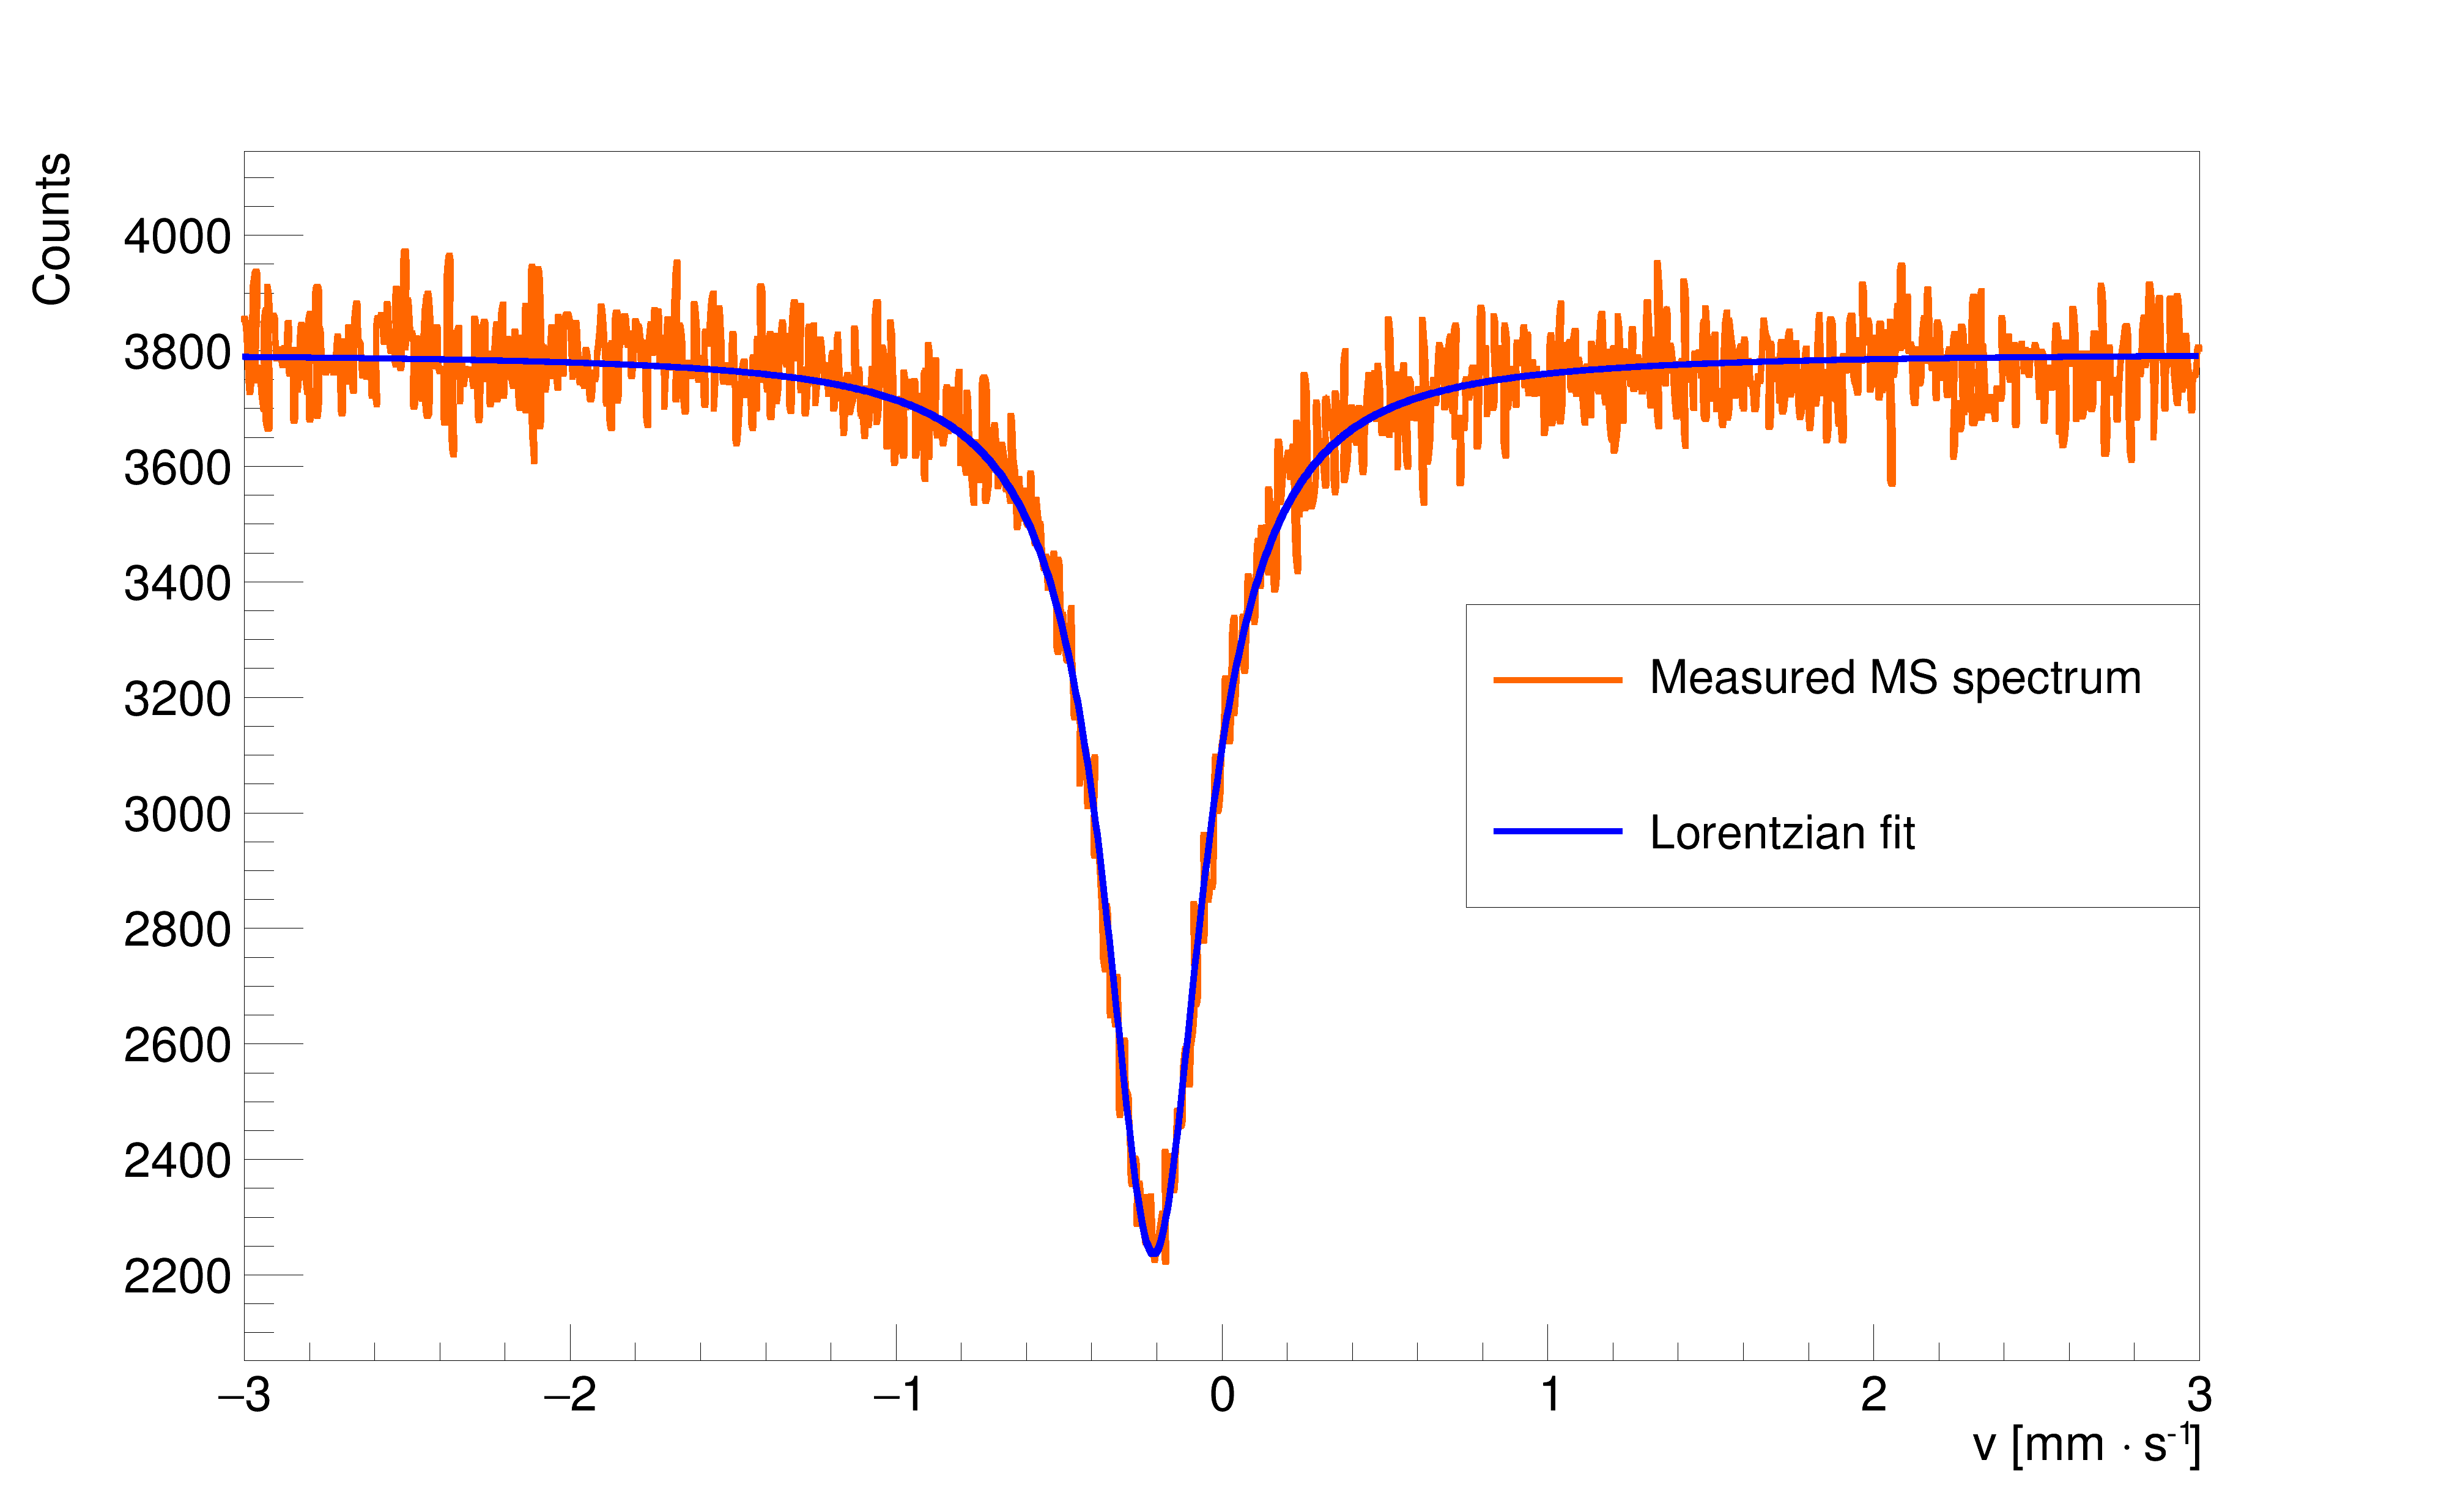
\includegraphics[scale=0.125, angle = 0]{./pictures/MossSemi.png}
\caption{Si PIN detector K$_{3}[$Fe(CN)$_{6}]$ MS spectra.}
\label{Si PIN detector MS spectra.}

\end{figure}

\begin{figure}[H]
\centering
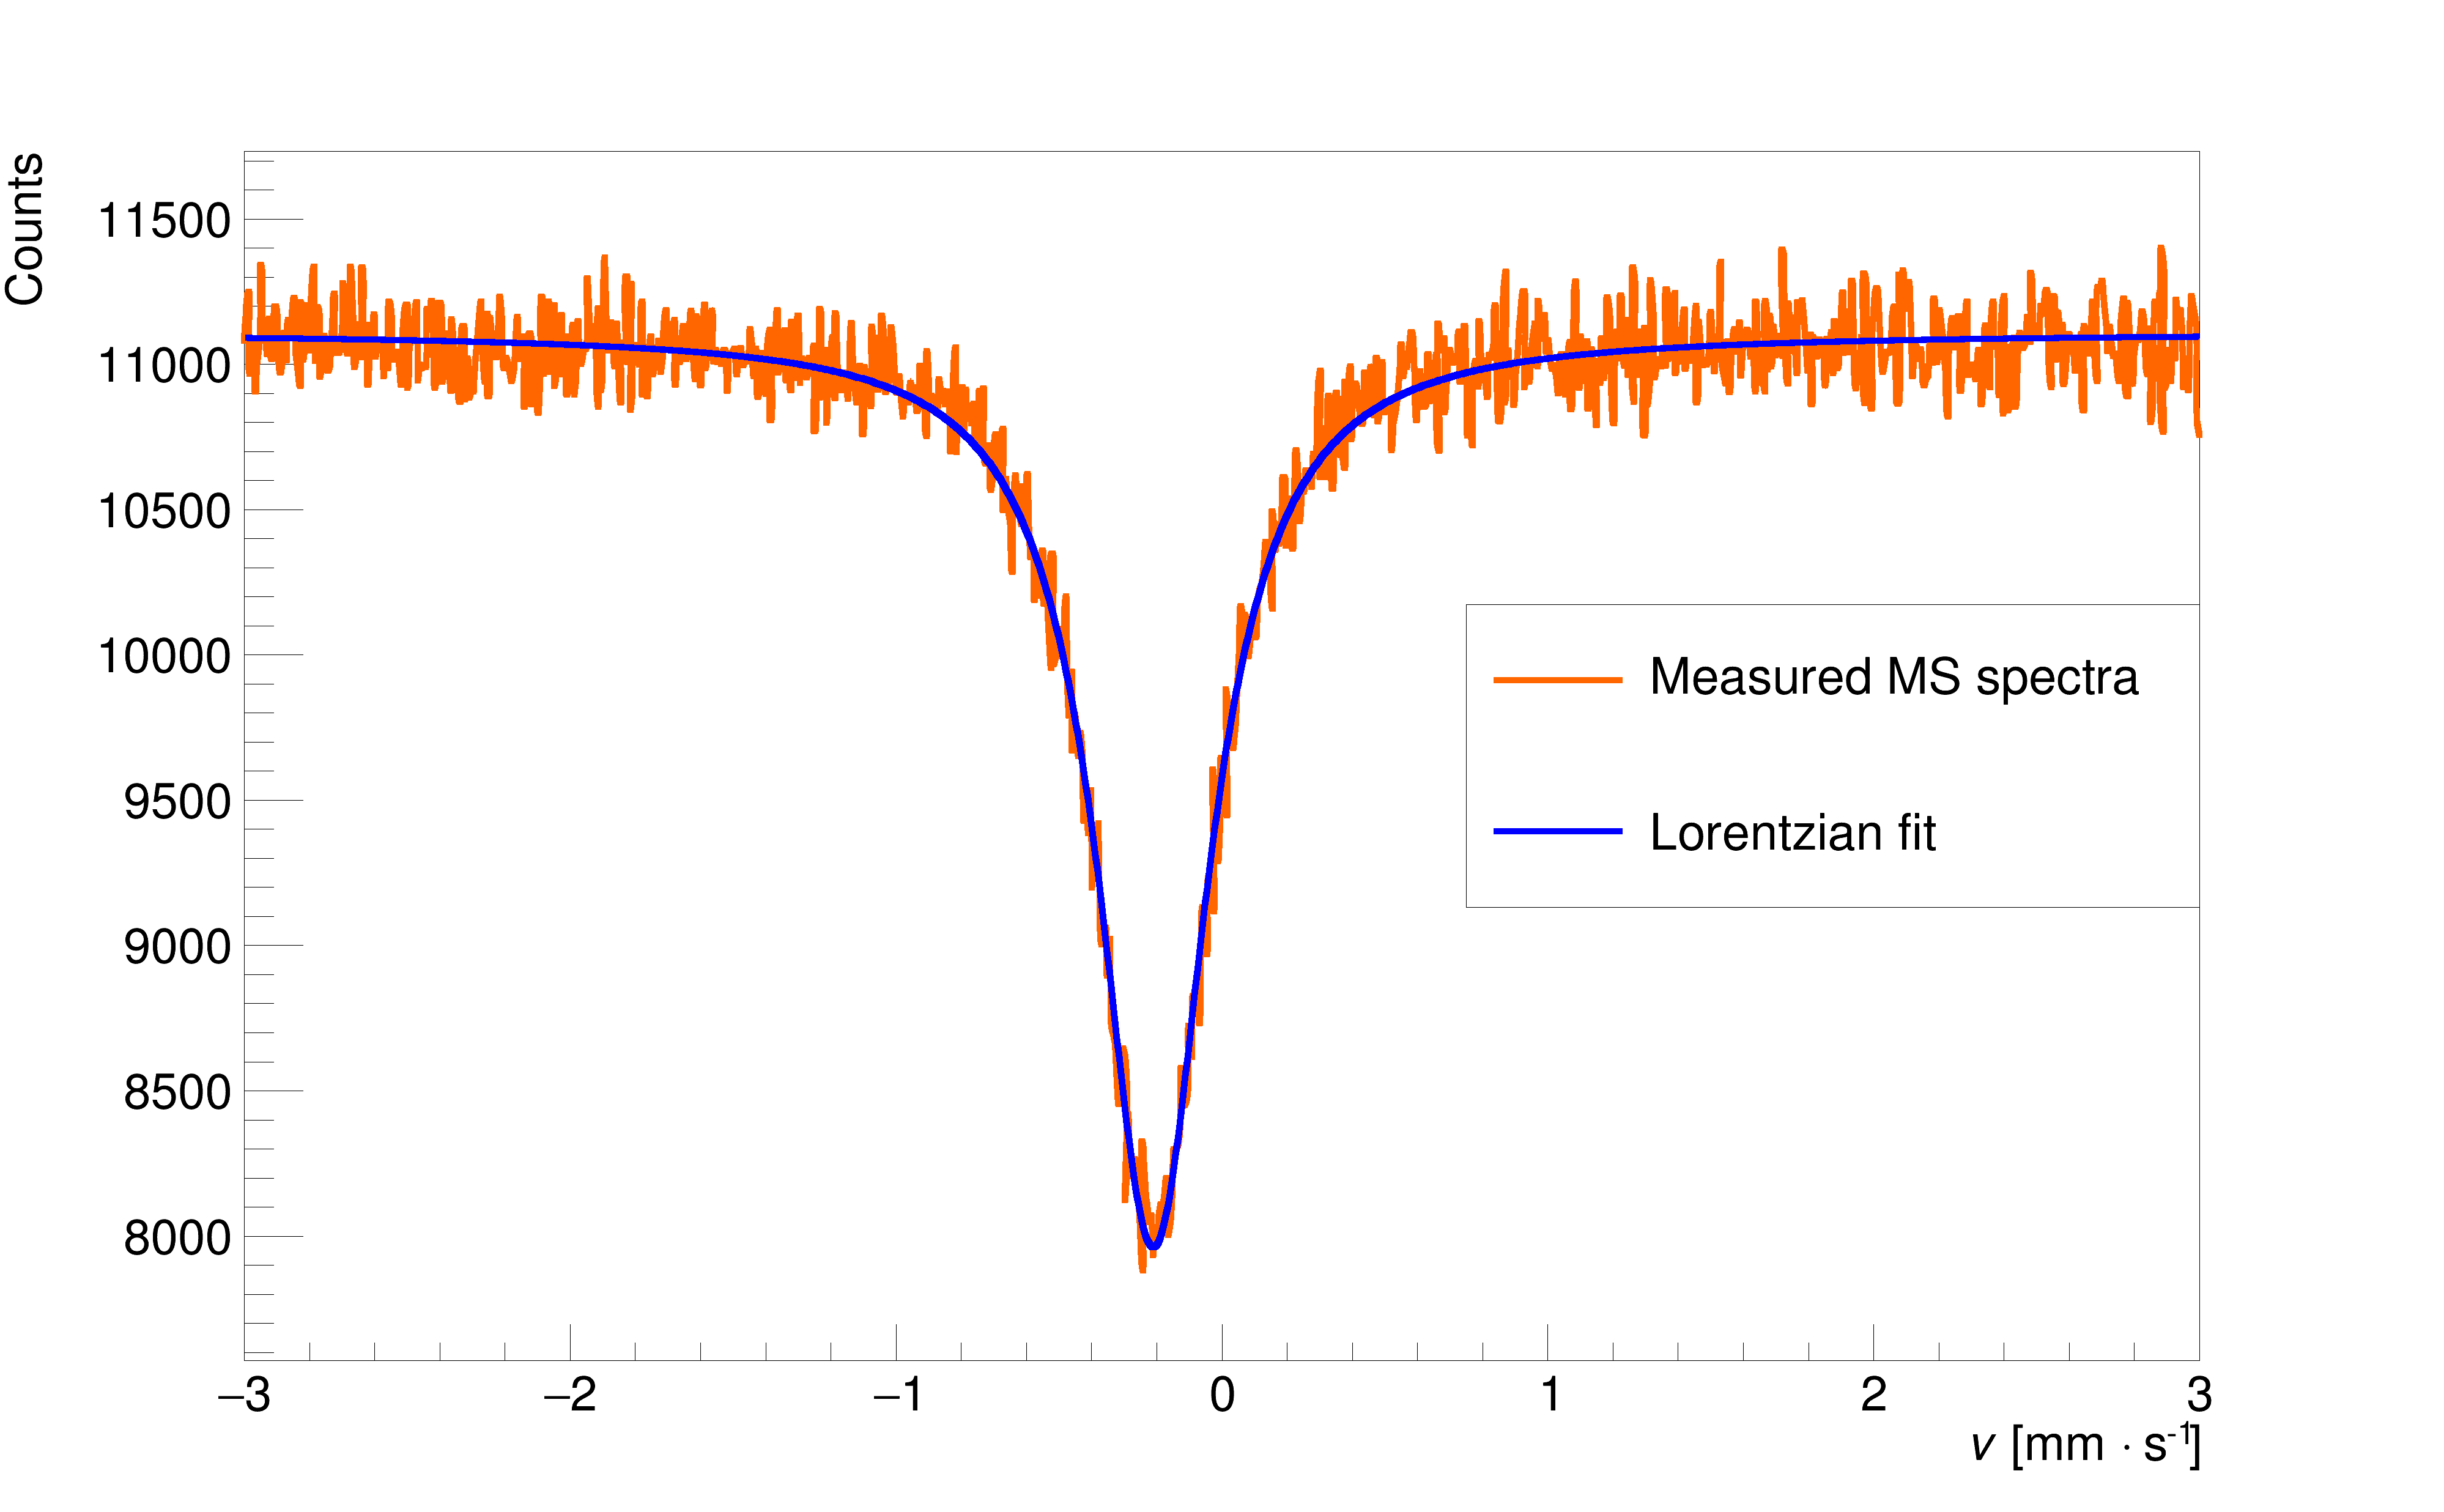
\includegraphics[scale=0.125, angle = 0]{./pictures/MossGas.png}
\caption{Gas detector K$_{3}[$Fe(CN)$_{6}]$ MS spectra.}
\label{Gas detector MS spectra.}

\end{figure}

\begin{figure}[H]
\centering
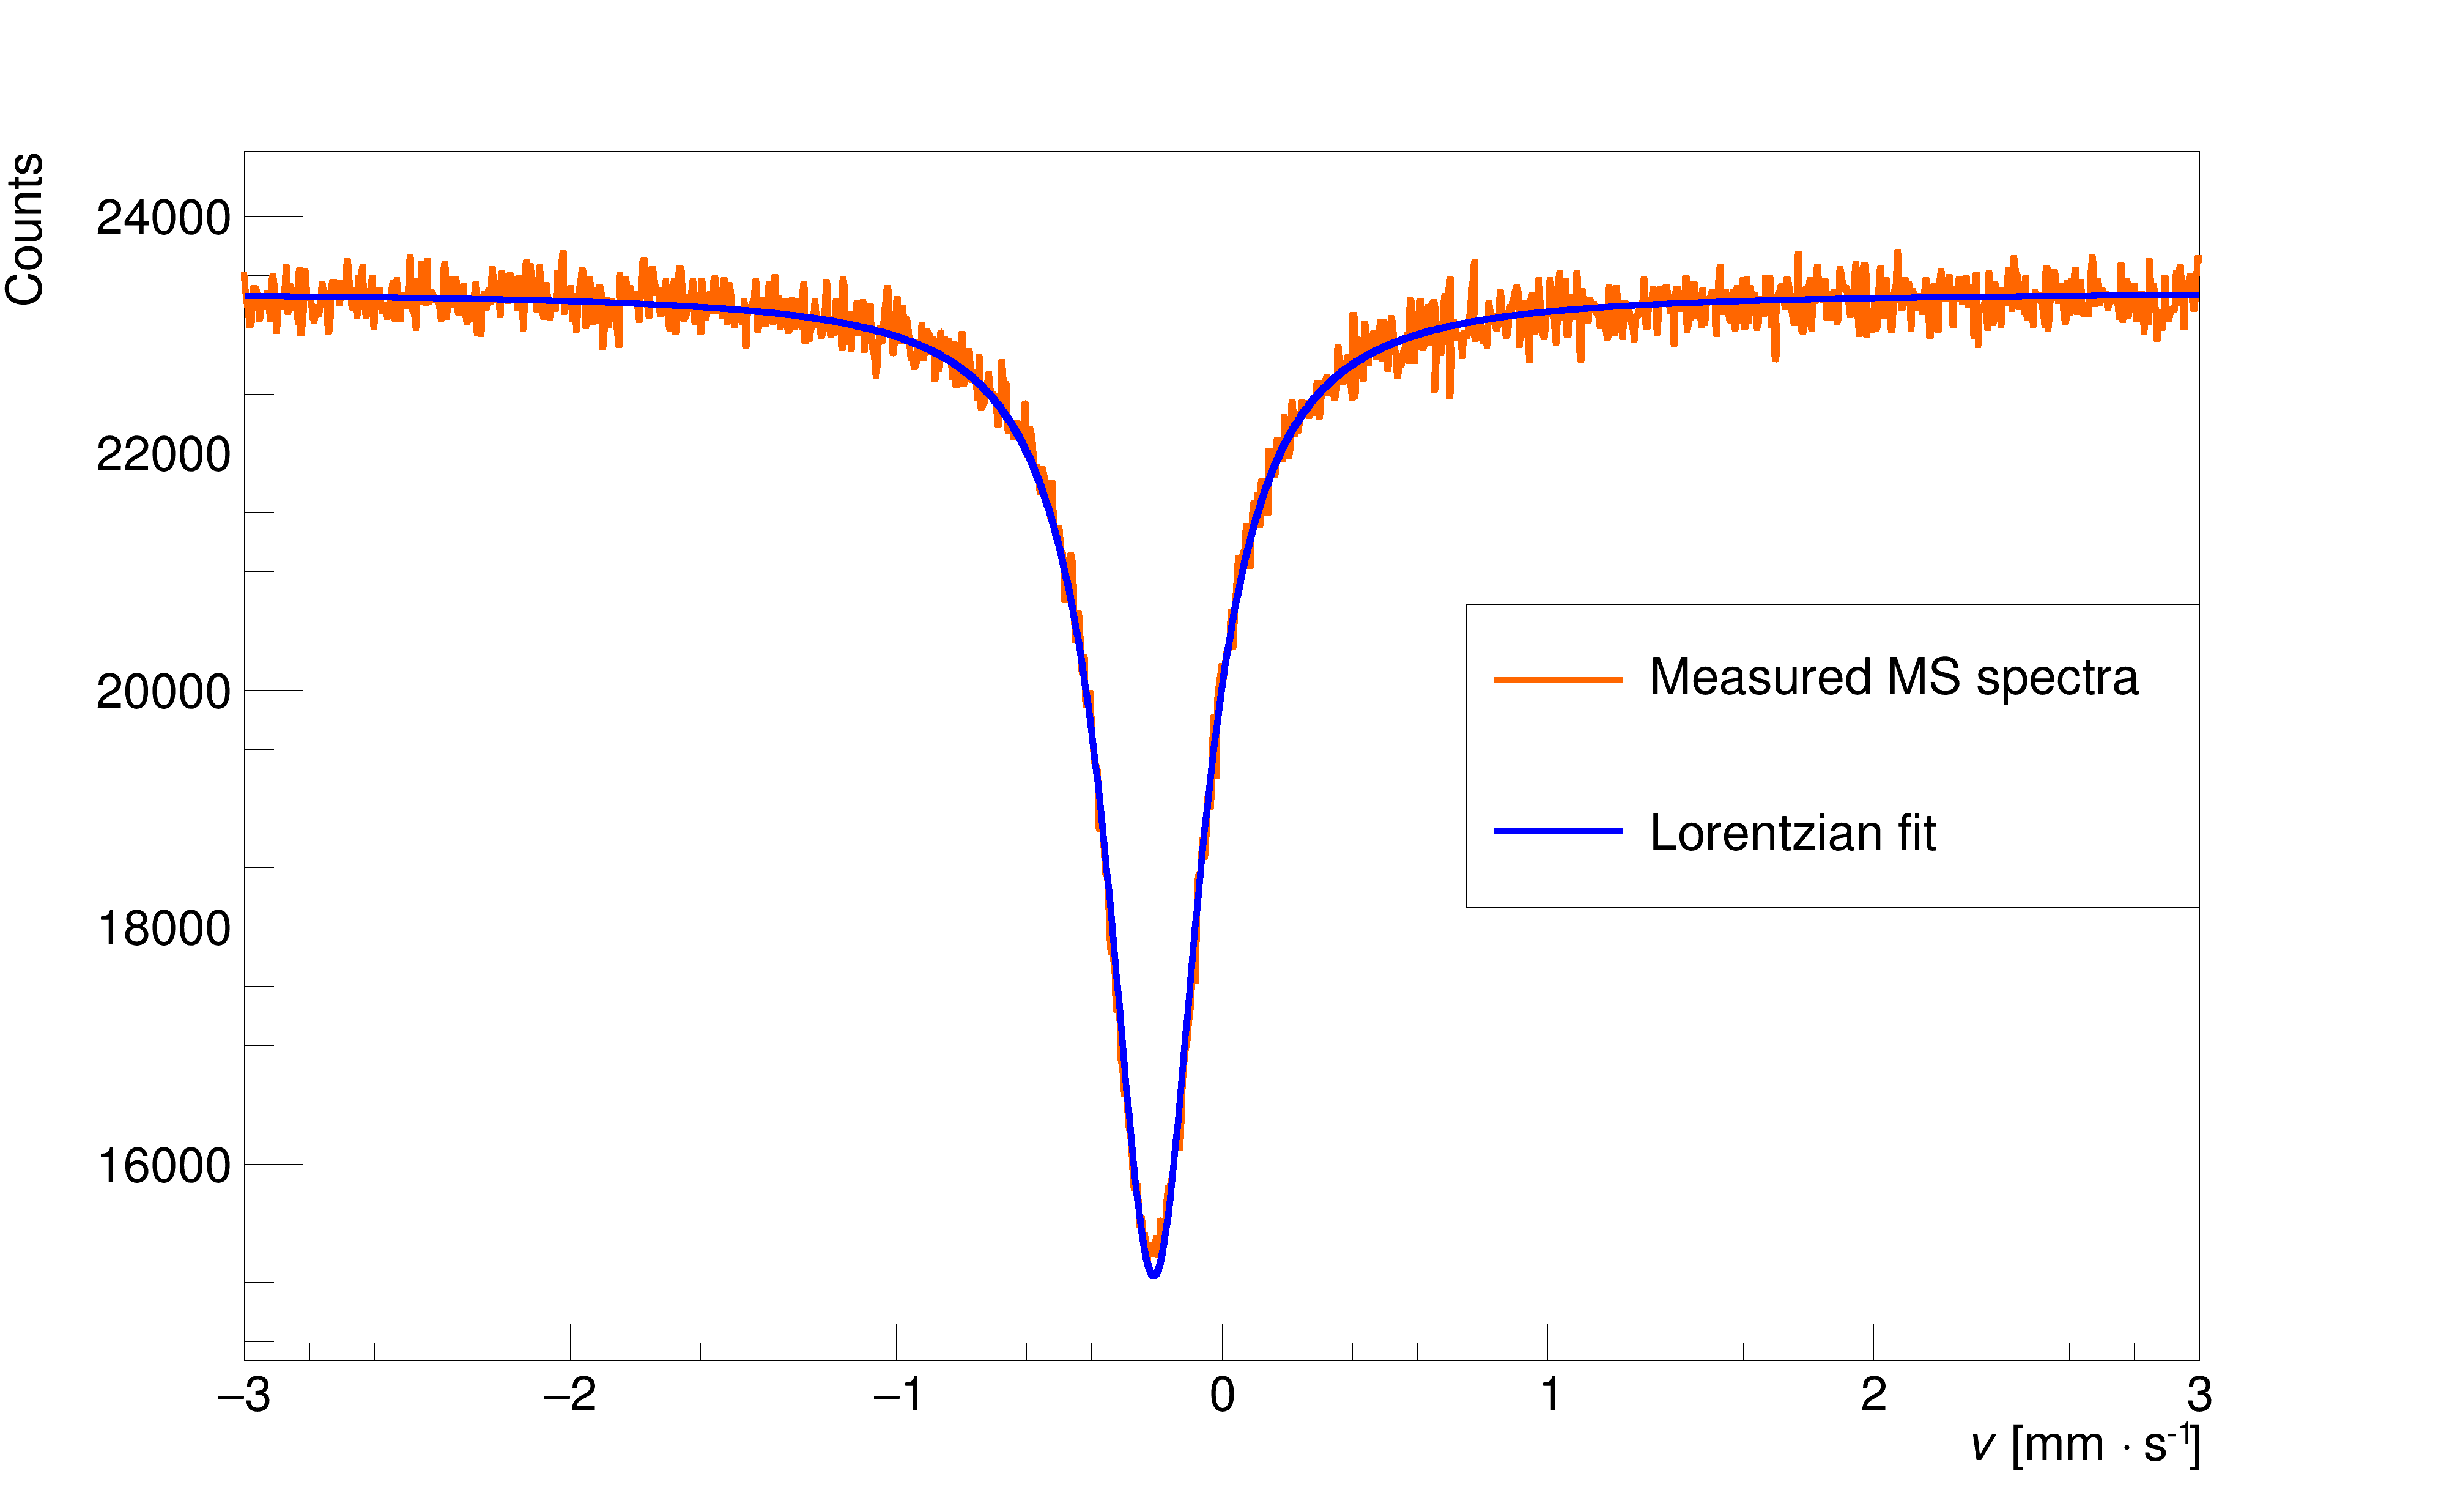
\includegraphics[scale=0.125, angle = 0]{./pictures/MossPMT.png}
\caption{Scintillator detector K$_{3}[$Fe(CN)$_{6}]$ MS spectra.}
\label{Scintillator detector MS spectra.}

\end{figure}


Every spectra is fitted by the Lorentzian in the form described by equation \ref{lor}. However, in order to compare the MS parameters between detectors, there was a problem with the different $\Gamma$ in every spectra, which is not caused by the detector, but probably by the transducer. If the SNR$_{\textrm{MS}}$ and $E_{\textrm{MS}}$ (equations \ref{SNR} and \ref{effect}), which both depend on $I$, are to be comparable between the measurements, it is necessary to recalculate the $I$ for every Lorentzian. The recalculation is based on the following consideration: The altered velocity signal can cause the variations in $\Gamma$ of a singlet Lorentzian curve, however, its area $A$ (total number of counts) given by equation \ref{area} should be left unchanged by this effect. So if the $A$ is conserved although the $\Gamma$ is changed, the new amplitudes $I_{\textrm{rec}}$ corresponding to the recalculated Lorentzians with the same $\Gamma_{\textrm{ref}}$  can be obtained by a simple relation $I_{\textrm{rec}} = \frac{\Gamma}{\Gamma_{\textrm{ref}}}I$. As a reference $\Gamma_{\textrm{ref}}$ is taken the smallest $\Gamma$ of the three detectors.
The results obtained for every detector can be seen in table \ref{mossres}.

\begin{table}[H]
\centering
\begin{tabular}{|c|c|c|}
\hline
   & SNR$_{\textrm{MS}}$ & $E_{\textrm{MS}}$ \\ \hline
Si PIN & $27.4 \pm 0.5$    & $0.444 \pm 0.007$  \\ \hline
gas & $35.7 \pm 0.5$    & $0.338 \pm 0.005$ \\ \hline
scintillator  & $54.3 \pm 0.3$    & $0.355 \pm 0.002$ \\ \hline
\end{tabular}
\caption{Measured SNR$_{\textrm{MS}}$ and $E_{\textrm{MS}}$ for every detector.}
 \label{mossres}
\end{table}

The results show that the best SNR$_{\textrm{MS}}$ has the scintillator detector, and thus when it comes to acquiring the MS spectra in transmission geometry, the Si PIN detector is not the best candidate. However, the highest $E_{\textrm{MS}}$ is associated with the Si PIN, and thus it can be employed in some applications where $E_{\textrm{MS}}$ is an important parameter. 


